\section{一维离散映射系统:帐篷映射}
帐篷映射(Tent Map),是一个一维分段的线性映射,因其函数图像类似帐篷而得名。其广泛运用在混沌加密系统中,并且在混沌扩频码的产生、混沌加密系统构造和混沌优选算法的实现中也经常被使用。

帐篷映射是定义在$x\in [0,1]$上的一维离散映射:
\begin{equation}
    x_{n+1}=f(x_n)=
    \begin{cases}
        \begin{aligned}
            &\dfrac{x_n}{\alpha}&,\ x\in [0,\alpha)\\
            &\dfrac{1-x_n}{1-\alpha}&,\ x\in [\alpha,1]
        \end{aligned}
    \end{cases},\ n=1,2,3,\cdots
\end{equation}
其中$0<\alpha<1$,在$\alpha=\frac{1}{2}$的特殊情况下,帐篷映射可以写为
\begin{equation}
    x_{n+1}=f(x_n)=1-2|x-\frac{1}{2}|=
    \begin{cases}
        \begin{aligned}
            &2x_n&,\ x\in [0,\frac{1}{2})\\
            &2-2x_n&,\ x\in [\frac{1}{2},1]
        \end{aligned}
    \end{cases},\ n=1,2,3,\cdots
\end{equation}

帐篷映射存在两个不动点:$x_1^*=0$和$x_2^*=\frac{2}{3}$。帐篷映射在其参数范围内是一个混沌映射,并且具有均匀的分布函数和良好的相关性。帐篷映射的相图描述了相空间的映射关系$x_n\rightarrow x_{n+1}$:
\begin{figure}
	\centering
	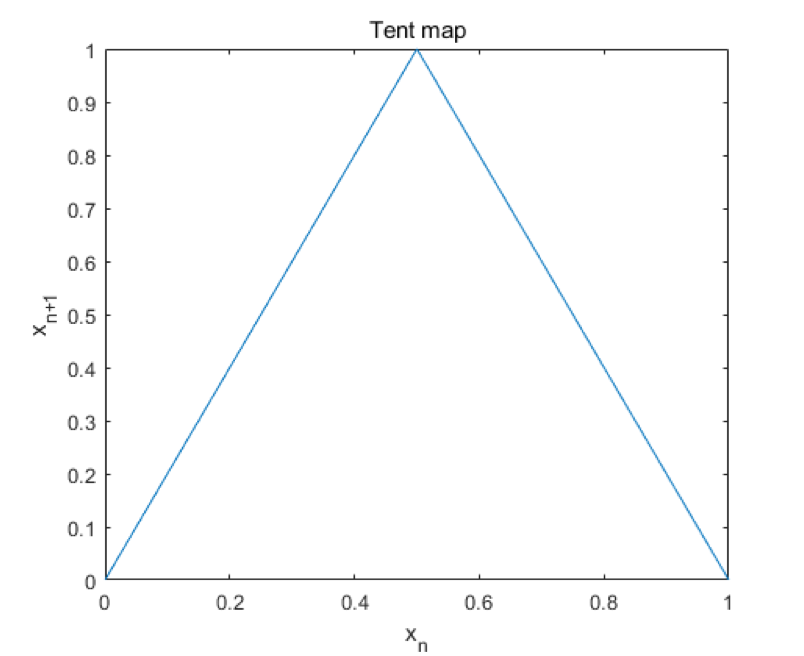
\includegraphics[scale=0.6]{tent_phase.png}
    \caption{帐篷映射的相图($\alpha=\frac{1}{2}$)}
    \label{fig:tent_pha}
\end{figure}